\chapter{Benutzerdokumentation}
\label{ch:4}

\section{Installation}
\subsection{Voraussetzungen}
F\"ur die Installation der Software ist ein Linux basiertes Betriebssystem, sowie die Vorinstallation von QT (Version 5) notwendig.

\subsection{Unkompilierte Version}
F\"ur die Installation der unkompilierten Version sind folgende Schritte zu befolgen:
\begin{enumerate}
  \item Erstellen eines gew\"unschten Installationsverzeichnisses, z.B. \verb+./Interpolation+
  \item Speichern von \verb+Interpolation.zip+ in dem gew\"ahlten Verzeichnis.
  \item Entpacken des Archivs mittels \verb+unzip Interpolation.zip+ oder einer entsprechenden Software.
  \item Ausf\"uhren von \verb+qmake-qt5+ in dem gew\"ahlten Verzeichnis.
  \item Anschlie\ss end ausf\"uhren von \verb+make+ in dem gleichen Verzeichnis.
  \item 'make clean' stellt den Ausgangszustand des Programms wieder her, erh\"alt aber die ausf\"uhrbare Datei.
  \item Ausf\"uhren des Programms durch das Starten der ausf\"uhrbaren Datei 'Interpolation'.
\end{enumerate}

\section{Beispielsitzung}
Das Programm startet mit der Anzeige des Hauptfensters.\\

\begin{figure}[H]
\centering
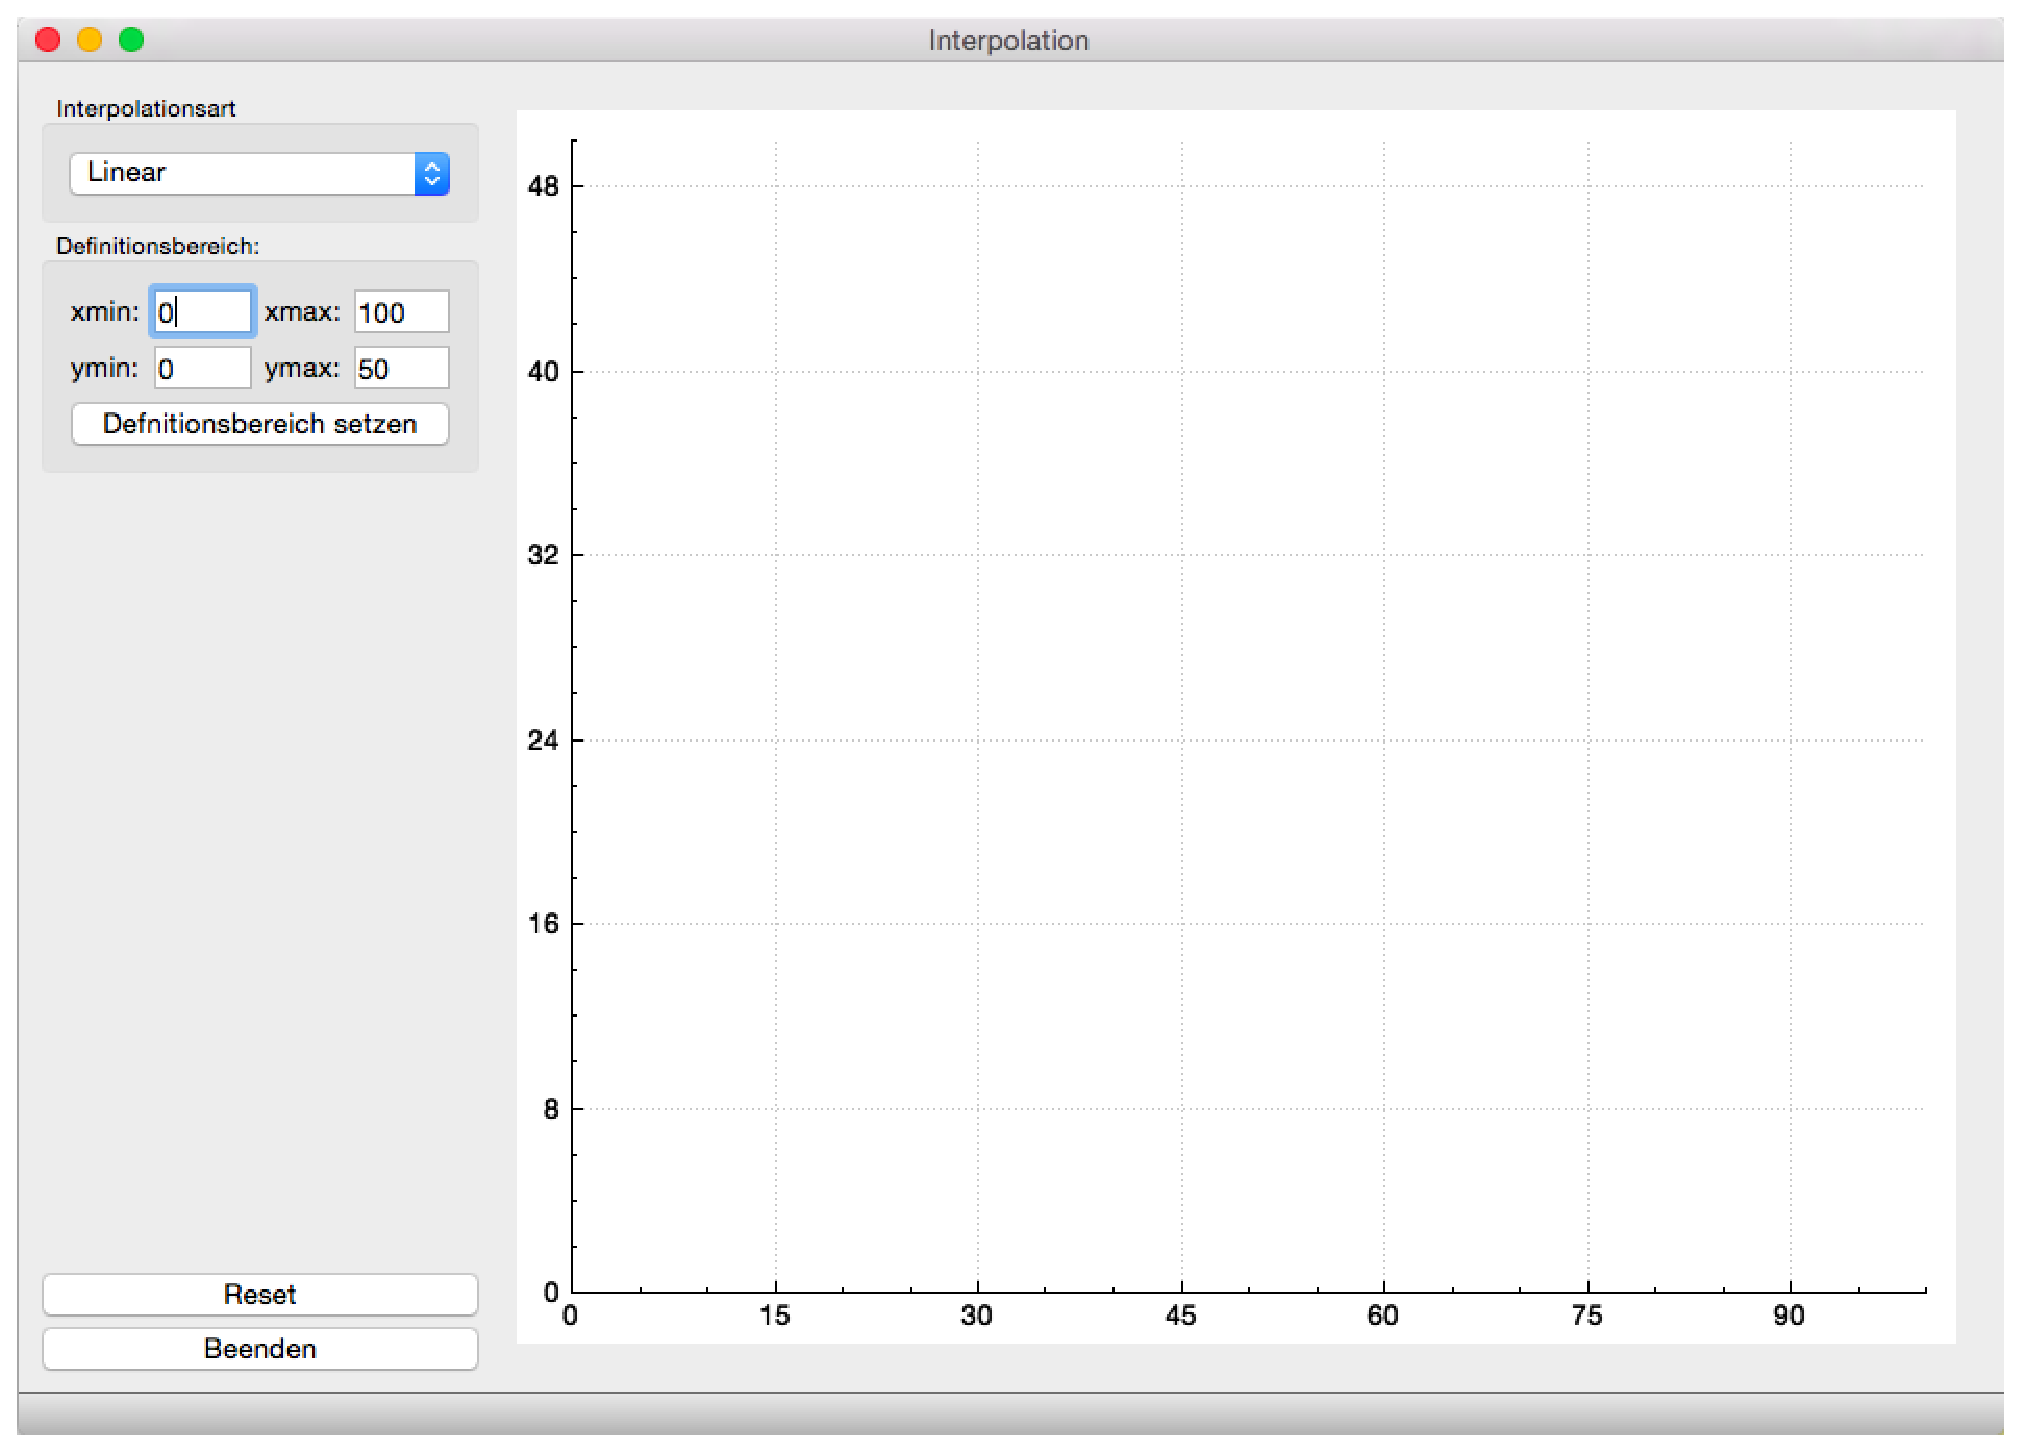
\includegraphics[width=\textwidth]{figures/start_screen.eps}
\caption{Startbildschirm}
\end{figure}

\noindent Der Nutzer klickt auf die Zeichenfl\"ache mehrmals um Punkte hinzuzuf\"ugen. Diese werden auf der Zeichenfl\"ache direkt angezeigt und durch gerade Linien (lineare Splines) verbunden.\\

\begin{figure}[H]
\centering
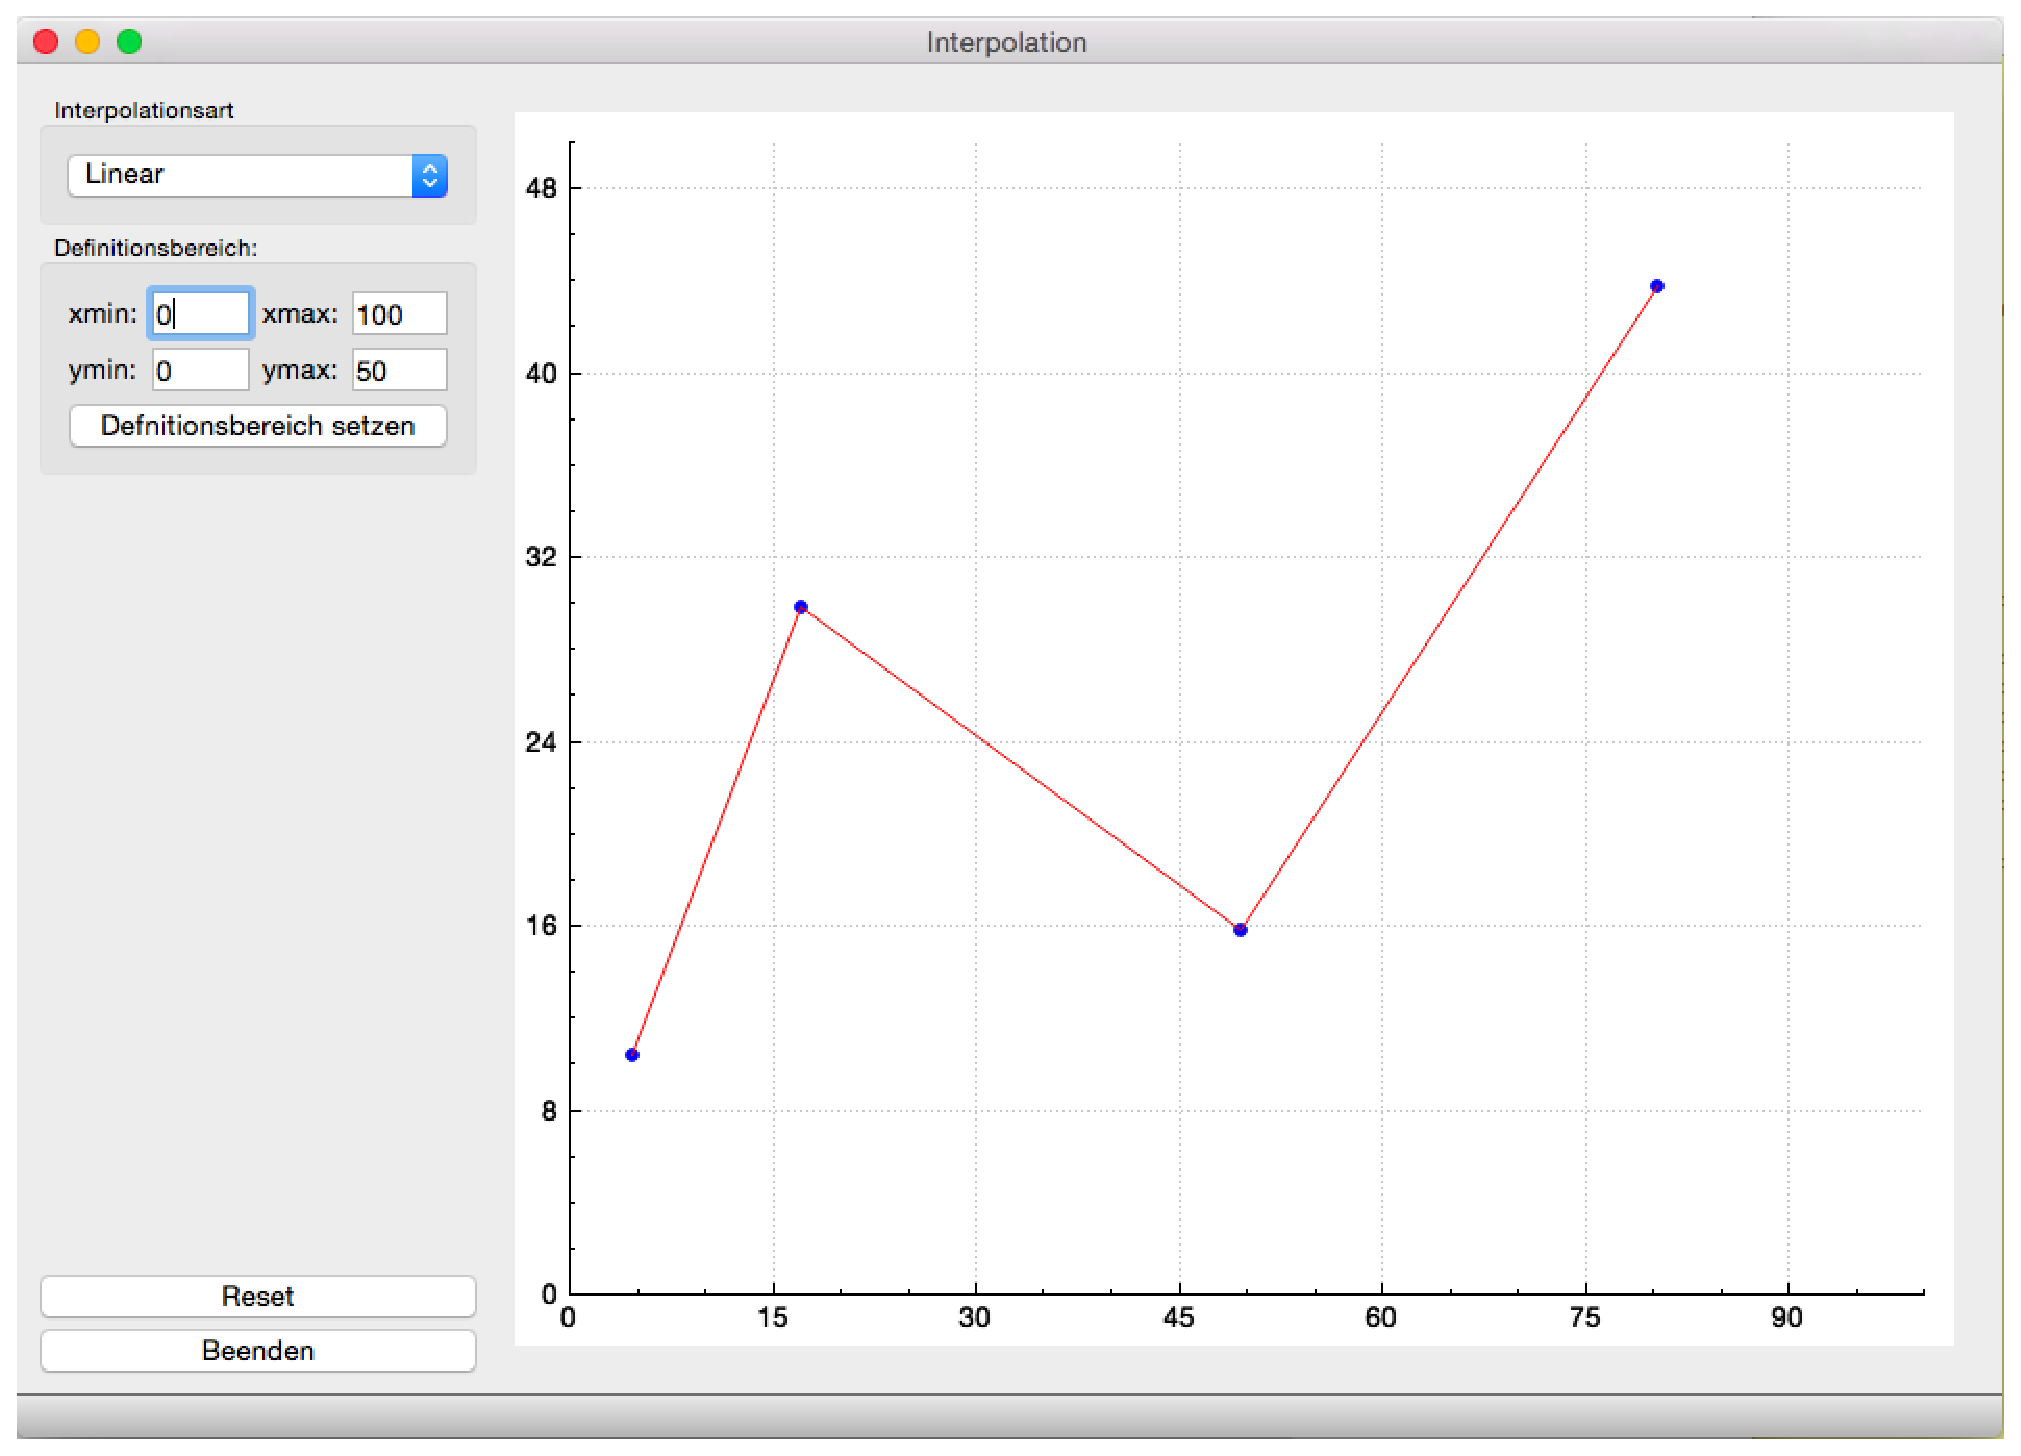
\includegraphics[width=\textwidth]{figures/linear_interpol_screen.eps}
\caption{Lineare Interpolation zwischen Punkten}
\end{figure}

\noindent Der Nutzer w\"ahlt die Interpolationsart 'Polynominterpolation' aus. Die Punkte werden nun durch eine Polynomkurve miteinander verbunden.\\

\begin{figure}[H]
\centering
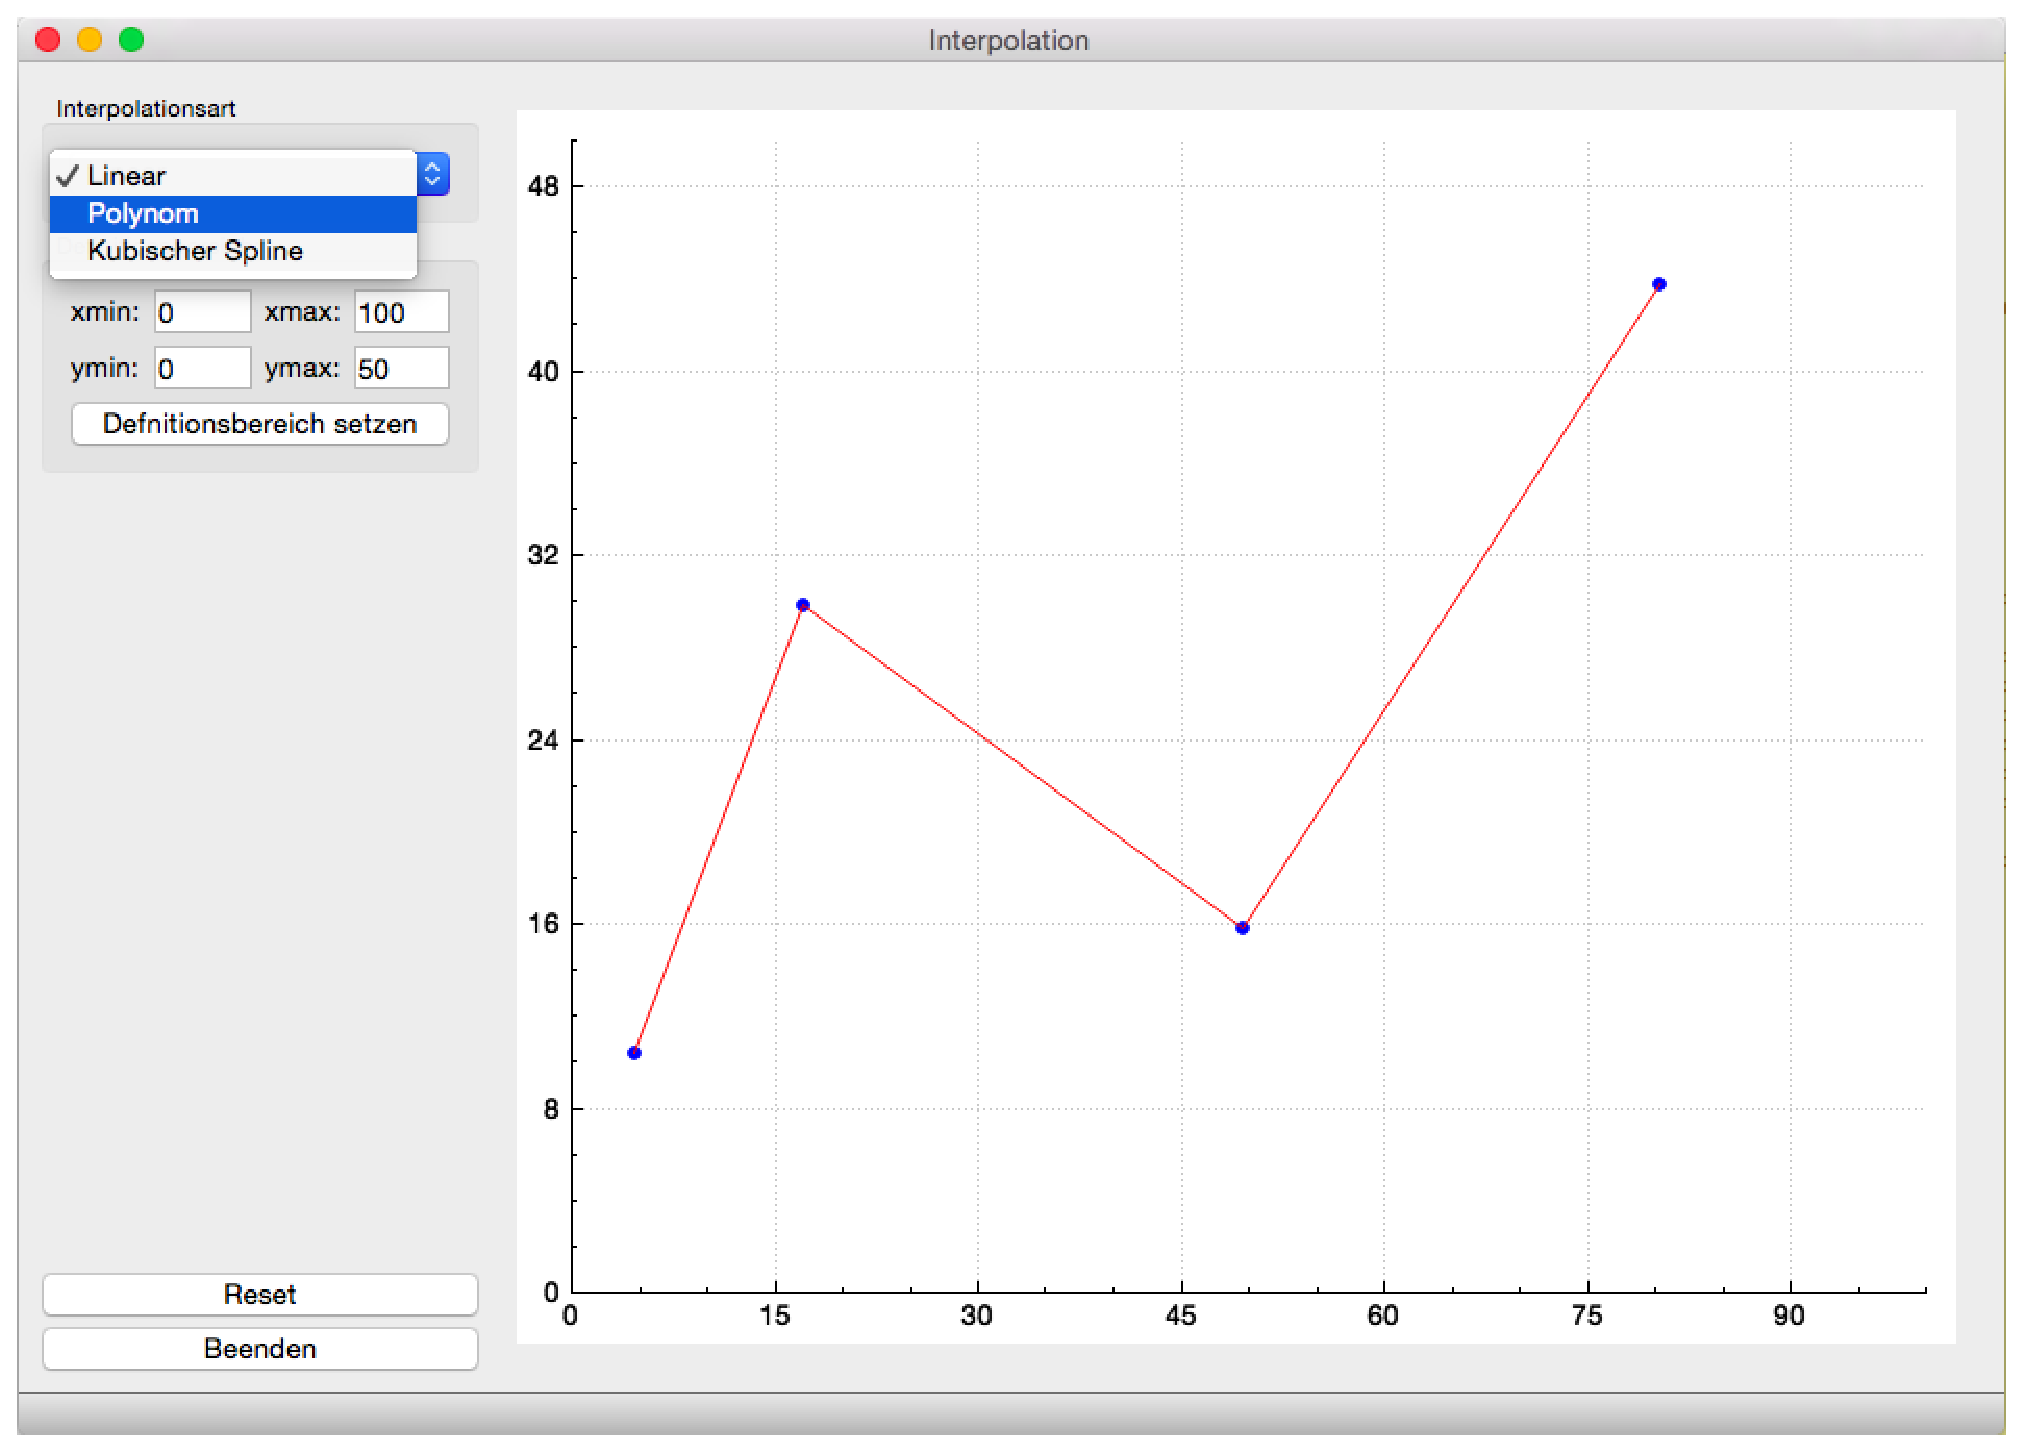
\includegraphics[width=\textwidth]{figures/change_interpol_screen.eps}
\caption{\"Andere Interpolationsart}
\end{figure}

\begin{figure}[H]
\centering
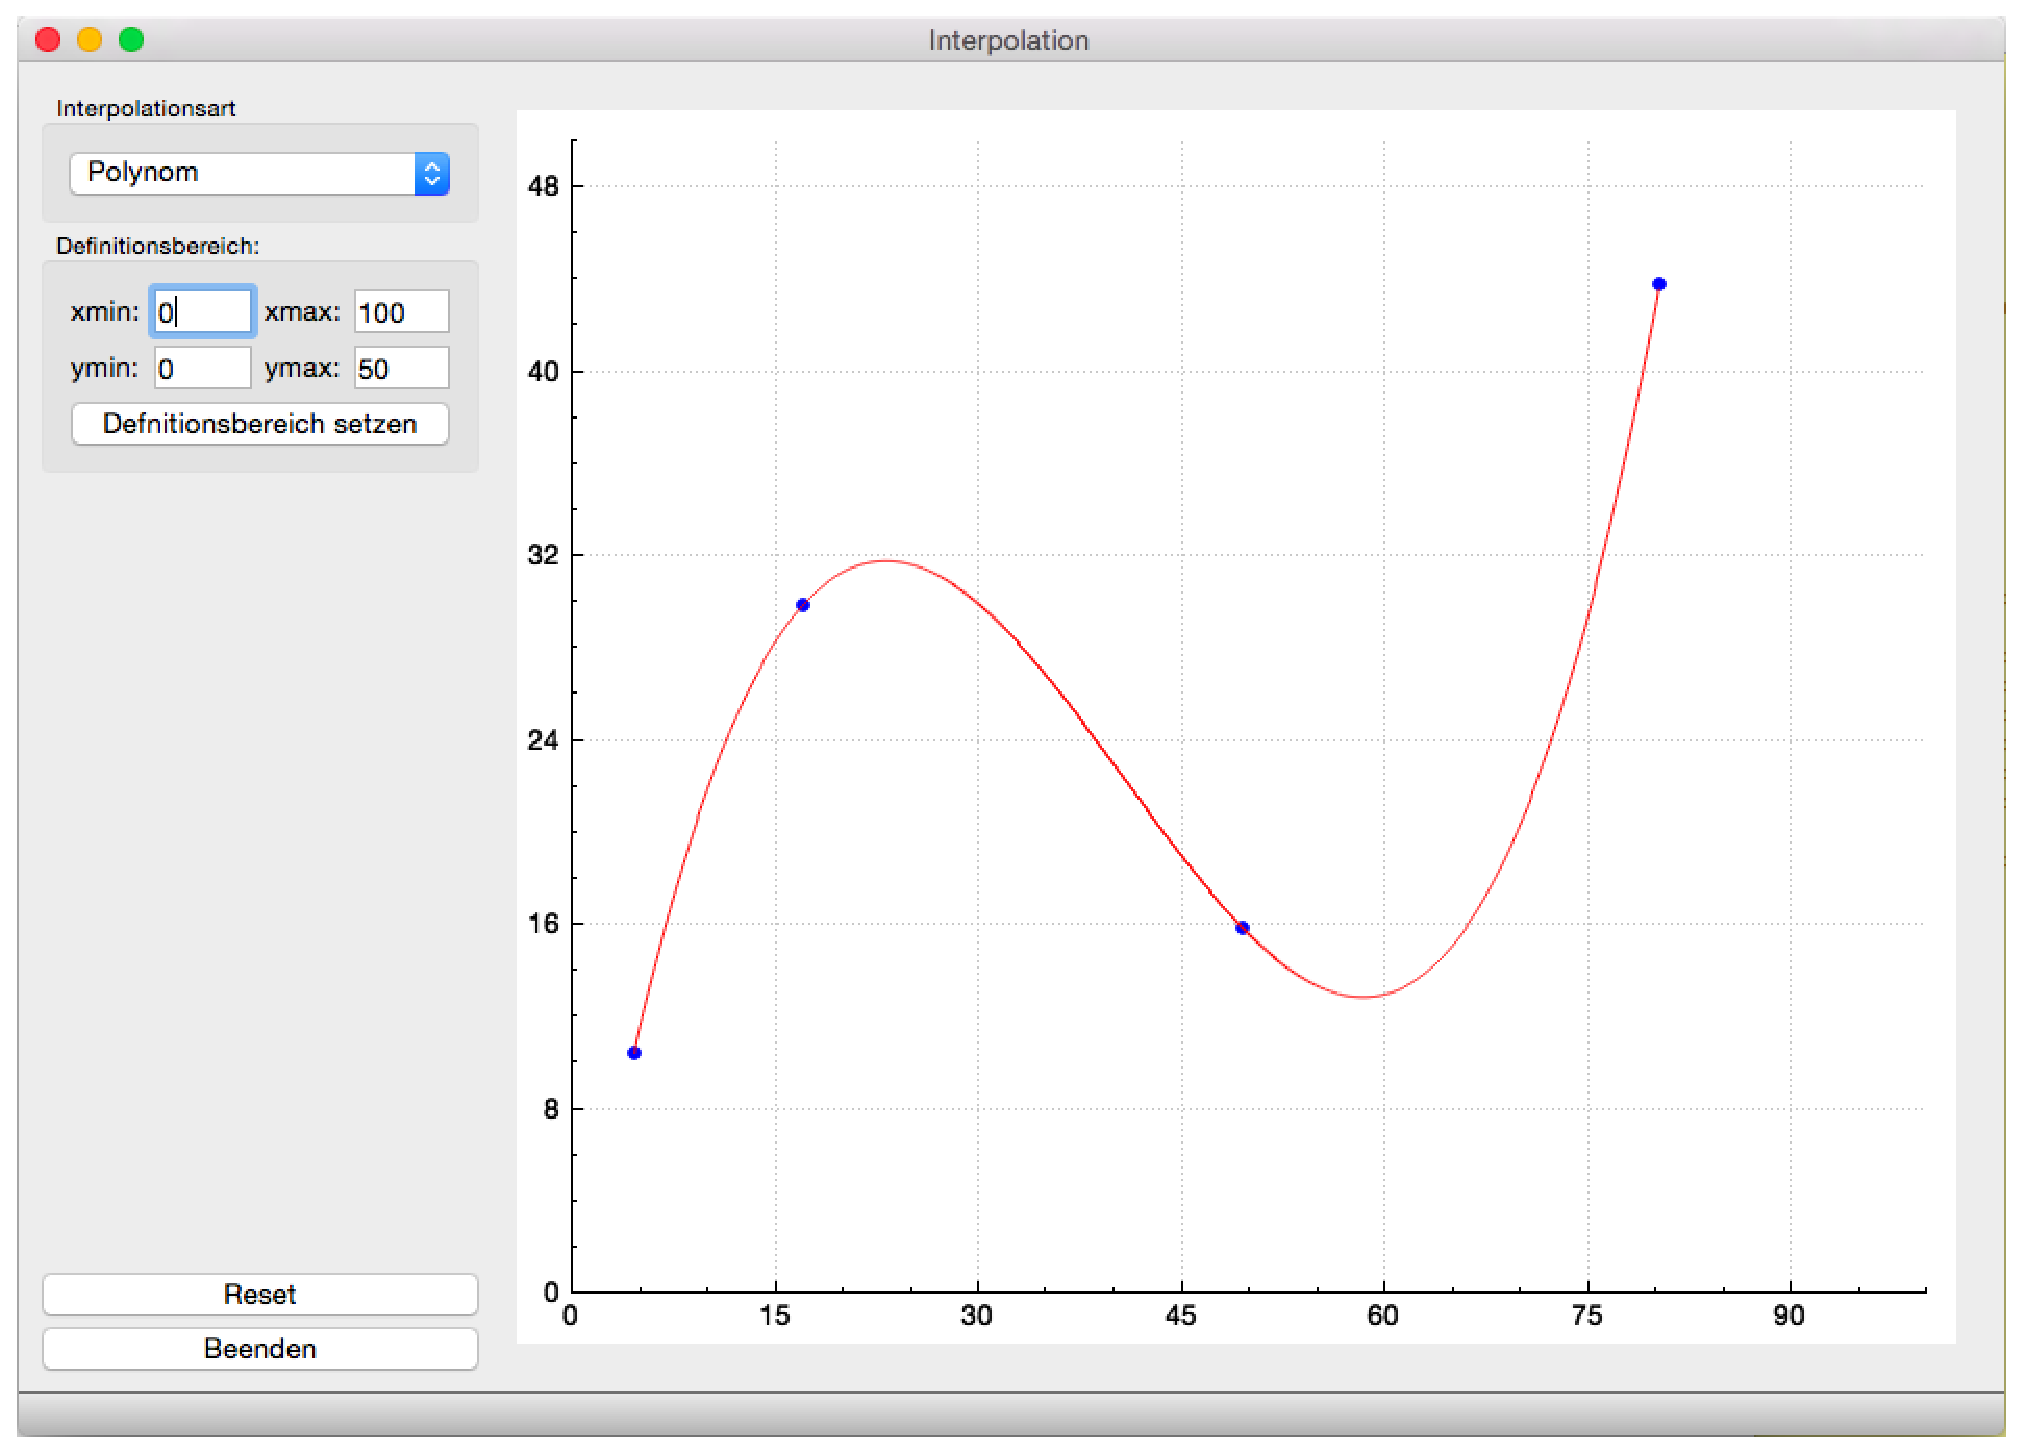
\includegraphics[width=\textwidth]{figures/polynom_interpol_screen.eps}
\caption{Polynominterpolation zwischen Punkten}
\end{figure}

\noindent Der Nutzer ver\"andert den Definitionsbereich durch Eingeben der Grenzen in die entsprechenden Textfelder und Klicken auf die Schaltfl\"ache 'Definitionsbereich setzen' . Sind die Grenzen jedoch nicht konform, d.h. ist xmin z.B. gr\"o\ss er als xmax, so wird eine Fehlermeldung ausgegeben.\\

\begin{figure}[H]
\centering
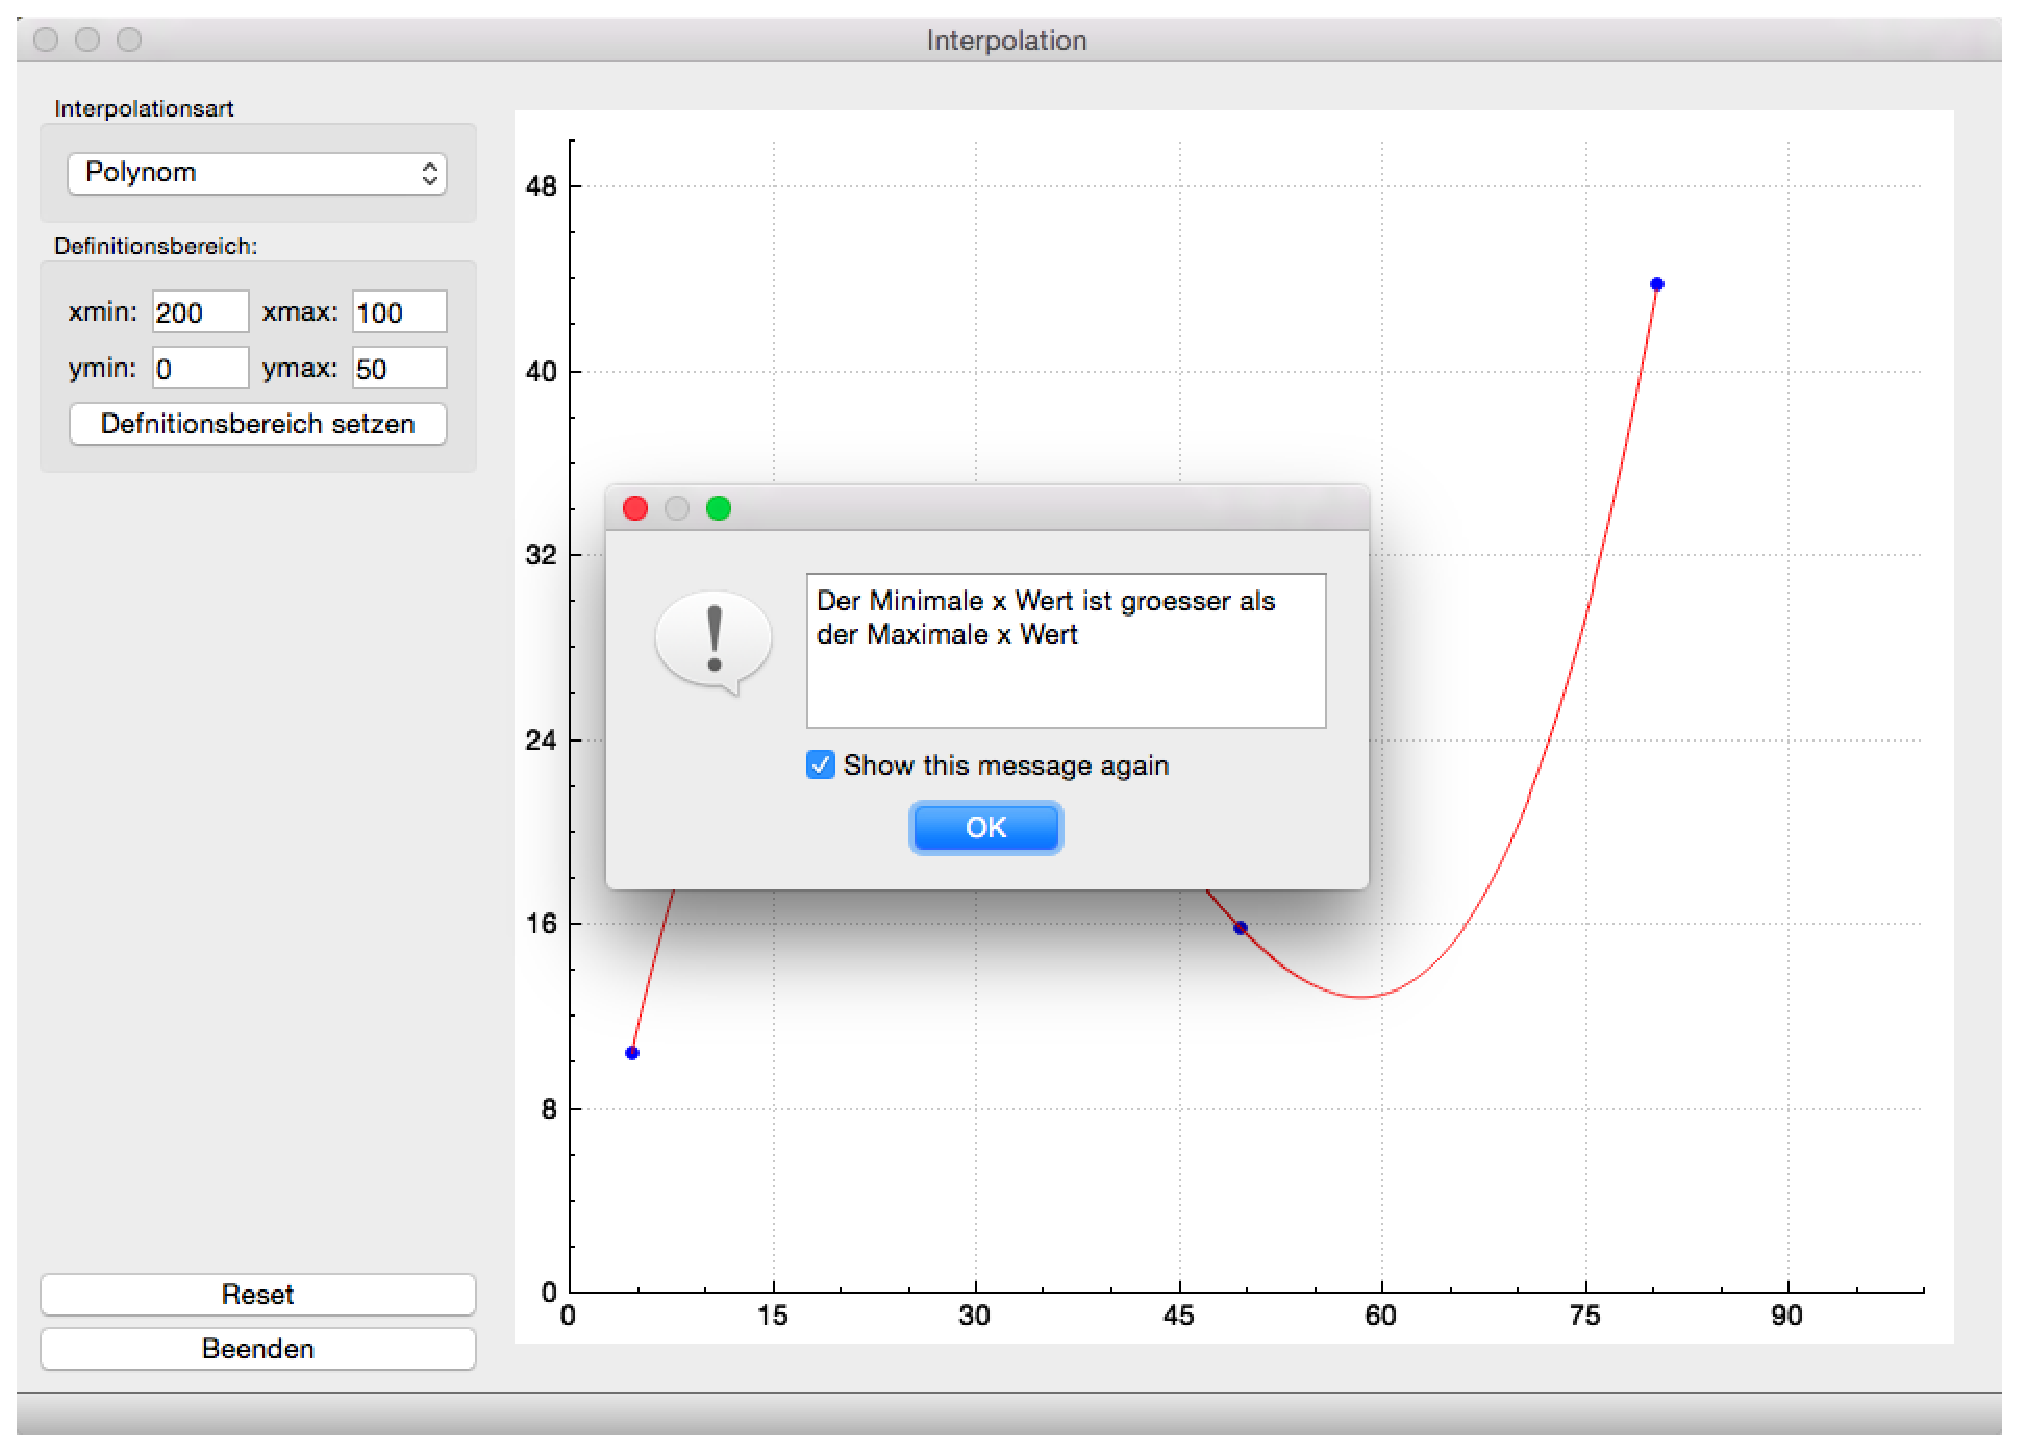
\includegraphics[width=\textwidth]{figures/error_message_screen.eps}
\caption{Anzeige einer Fehlermeldung}
\end{figure}

\noindent Der Nutzer klickt auf die Schaltfl\"ache 'Beenden' und das Programm schlie\ss t. 

\section{Fehlersituationen}
Das Programm gibt Fehlermeldungen aus. Diese k\"onnen nur entstehen, wenn der Definitionsbereich ver\"andert wird. Es wird eine Fehlermeldung ausgegeben, wenn ein Feld leer ist, einen Buchstaben enth\"alt, die Grenzen au\ss erhalb eines vordefinierten Intervalls oder die Anzahl der Nachkommastellen zu gro\ss \ ist. Es sind alle anderen Ausnahmen und m\"ogliche Fehlersituationen so behandelt, dass diese nicht angezeigt werden m\"ussen und sich der Benutzer komplett mit der Bedienung des Programms besch\"aftigen kann. Sollten dennoch Fehler auftreten bitten wir diese an stefan.jeske@rwth-aachen.de zu melden. 





